\documentclass{standalone}
\usepackage{tikz}
\usepackage{pgfplots}

\usetikzlibrary{positioning,intersections,calc,fadings,decorations.pathreplacing,decorations.markings}
\usetikzlibrary{shapes,arrows}
% ------------------------------------------------------------------------------------
% Chapter 1
% ------------------------------------------------------------------------------------

\newcommand{\Spitzer}{\textit{Spitzer}\xspace}
\newcommand{\WISE}{WISE\xspace}
\newcommand{\Herschel}{\textit{Herschel}\xspace}
\newcommand{\JWST}{JWST\xspace}
\newcommand{\OPD}{\ensuremath{\textrm{OPD}}\xspace}
\newcommand{\Lc}{\ensuremath{L_c}\xspace}


\newlength\mylen
\settowidth\mylen{\textbullet}
\addtolength\mylen{-3mm}

\newcommand{\Pext}{\ensuremath{P_\textrm{ext}}\xspace}
\newcommand{\Mcrit}{\ensuremath{M_\textrm{crit}}\xspace}
\newcommand{\tff}{\ensuremath{\textrm{t}_\textrm{ff}}\xspace}
\newcommand{\ts}{\ensuremath{\textrm{t}_\textrm{s}}\xspace}
\newcommand{\cs}{\ensuremath{c_\textrm{s}}\xspace}
\newcommand{\lambdaJ}{\ensuremath{\lambda_\textrm{J}}\xspace}
\newcommand{\MJ}{\ensuremath{M_\textrm{J}}\xspace}

\newcommand{\foverlap}{\ensuremath{f_\textrm{overlap}}\xspace}
\newcommand{\Vloss}{\ensuremath{V_\textrm{loss}}\xspace}
\newcommand{\sigWFE}{\ensuremath{\sigma_\textrm{WFE}}\xspace}
\newcommand{\sigOPD}{\ensuremath{\sigma_\textrm{OPD}}\xspace}
\newcommand{\sigtt}{\ensuremath{\sigma_\textrm{tt}}\xspace}
\newcommand{\renv}{\ensuremath{r_\textrm{env}}\xspace}
\newcommand{\Menv}{\ensuremath{M_\textrm{env}}\xspace}
\newcommand{\Mdotenv}{\ensuremath{\dot{M}_\textrm{env}}\xspace}
\newcommand{\Lbol}{\ensuremath{L_\textrm{bol}}\xspace}
\newcommand{\Tbol}{\ensuremath{T_\textrm{bol}}\xspace}
\newcommand{\Av}{\ensuremath{A_V}\xspace}

\newcommand{\Knu}{\ensuremath{\kappa_\nu}\xspace}
\newcommand{\Bnu}{\ensuremath{B_\nu}\xspace}
\newcommand{\Fnu}{\ensuremath{F_\nu}\xspace}
\newcommand{\Snu}{\ensuremath{S_\nu}\xspace}
\newcommand{\ext}{\ensuremath{\textrm{ext}}\xspace}
\newcommand{\Cext}{\ensuremath{C_\ext}\xspace}
\newcommand{\dust}{\ensuremath{\textrm{dust}}\xspace}

\newcommand{\QE}{\ensuremath{\textrm{QE}}\xspace}
\newcommand{\MDLF}{\ensuremath{\textrm{MDLF}}\xspace}
\newcommand{\MDFD}{\ensuremath{\textrm{MDFD}}\xspace}
\newcommand{\Tint}{\ensuremath{T_\textrm{int}}\xspace}
\newcommand{\Nscan}{\ensuremath{N_\textrm{scan}}\xspace}
\newcommand{\Smin}{\ensuremath{S_\textrm{min}}\xspace}
\newcommand{\Rnir}{\ensuremath{R_\textrm{NIR}}\xspace}
\newcommand{\sigRON}{\ensuremath{\sigma_\textrm{RON}}\xspace}
\newcommand{\Nph}{\ensuremath{N_\textrm{ph}}\xspace}
\newcommand{\Nel}{\ensuremath{N_{\textrm{e}^-}}\xspace}
\newcommand{\FBW}{\ensuremath{\textrm{FBW}}\xspace}


\newcommand{\sigman}{\ensuremath{\sigma^\textrm{man}}\xspace}
\newcommand{\sigstd}{\ensuremath{\sigma^\textrm{std}}\xspace}
\newcommand{\sigth}{\ensuremath{\sigma^\textrm{th}}\xspace}

\newcommand{\Rpercent}{\ensuremath{R_{\%}}\xspace}
\newcommand{\Rfifty}{\ensuremath{R_{50}}\xspace}

\newcommand{\Rstar}{\ensuremath{R_{\star}}\xspace}
\newcommand{\Fmod}{\ensuremath{F_\textrm{mod}}\xspace}
\newcommand{\Fobs}{\ensuremath{F_\textrm{obs}}\xspace}
\newcommand{\Mstar}{\ensuremath{M_{\star}}\xspace}
\newcommand{\Tstar}{\ensuremath{T_{\star}}\xspace}
\newcommand{\Lstar}{\ensuremath{L_{\star}}\xspace}
\newcommand{\Rdiskmax}{\ensuremath{R_\textrm{disk}^\textrm{max}}\xspace}
\newcommand{\Rdiskmin}{\ensuremath{R_\textrm{disk}^\textrm{min}}\xspace}
\newcommand{\Mdisk}{\ensuremath{M_\textrm{disk}}\xspace}
\newcommand{\Renvmax}{\ensuremath{R_\textrm{env}^\textrm{max}}\xspace}
\newcommand{\Renvmin}{\ensuremath{R_\textrm{env}^\textrm{min}}\xspace}


% ------------------------------------------------------------------------------------
% Chapter 2
% ------------------------------------------------------------------------------------

% Units
\def\um{\si{\micro\meter}}
%\newcommand{\um}{\si{\micro\meter}}

\def\asec{\textrm{arcsec}}
\def\cm1{\ensuremath{\textrm{cm}^{-1}}}

%angle definitonis
\def\shat0{\hat{\textbf{s}}_0}
%\def\Ds{\Delta\textbf{s}}
\def\Ds{\xi}
\def\urad{\ensuremath{\mu\textrm{rad}}}

% Interferogram notations
\def\samp{s}
\def\baseline{\mathbf{B}}
\def\Bspec{B}
\def\F{\mathcal{F}}
\def\I{\textit{I}}
\def\Im{\I_\textrm{measured}}
\def\mI{\mathcal{I}}
\def\xn{x_n}
\def\xnp{x_{n'}}
\def\pxn{(\xn)}
\def\pxnp{(\xnp)}
\def\Ixn{\mI\pxn}
\def\Ikxn{\mI_k\pxn}
\def\Iksxn{\mI_k^{*}\pxnp}
\def\Vb{\mathcal{V}_\baseline}
\def\Phib{\Phi_\mathbf{B}}
\def\Phibp{\Phi_\textrm{bp}}
\def\Vi{\mathcal{V}_\textrm{i}}
\def\Phii{\Phi_\mathbf{i}}
\def\V{\mathcal{V}}
\def\S{\mathcal{S}}
\def\R{\mathcal{R}}
\def\oS{\overline{\S}}
\def\etaBS{\eta_{\textrm{b}}}
\def\etamf{\eta_\textrm{mf}}
\def\etao{\eta_o}
\def\s{\sigma}
\def\sig{\Delta}
\def\ps{(\s)}
\def\pms{(-\s)}
\def\Be{\B_e}
\def\Phir{\Phi_r}
\def\etaD{\eta_D}
\def\Tbp{\mathcal{T}_\textrm{bp}}
\def\Area{\mathcal{A}}
\def\F{\mathcal{F}}
\def\Ahat{\hat{\mathcal{A}}}
\def\Dx{dx}
\def\Dt{dt}
\def\D{d}
\def\intinf{\int_{-\infty}^{+\infty}}
\def\sinc{\textrm{sinc}}
\def\real{\textrm{Re}}
\def\imag{\textrm{Im}}
\def\FT{\mathcal{F}}
\def\DFT{\mathbf{DFT}}
\def\dsig{\delta\s}
\def\varPhir{\sig^2_\Phi}
\def\sigPhir{\sig_\Phi}
\def\Dopd{\sig_{\textrm{OPD}}}
\def\varopd{\sig^2_{\textrm{OPD}}}
\def\wk{w_k}
\def\O{\mathcal{O}}

% Noise definitons
\def\SNR{\ensuremath{\textrm{SNR}}\xspace}
\def\SNRnp{\SNR_\textrm{np}}
\def\ni{n_\mI}
\def\nA{n_+}
\def\nB{n_-}
\def\NEP{\textrm{NEP}}
\def\NEPtot{\NEP_\textrm{tot}}
\def\NEPph{\NEP_\textrm{ph}}
\def\NEPdet{\NEP_\textrm{det}}
\def\NEPsou{\NEP_\textrm{sou}}
\def\VAR{\mathbf{VAR}}
\def\varI{\sig_\mI^2}
\def\sigI{\sig_\mI}
\def\varspec{\sig_\mathcal{S}^2}
\def\varspectot{\sig^2_{\mathcal{S}\textrm{,tot}}}
\def\sigspec{\sig_\mathcal{S}}
\def\sigk{\s_k}
\def\mK{\mathcal{K}}
\def\sigalpha{\sig_\alpha}
\def\sigL{\sig_L}



\def\delay{\delta}
\def\delaytot{\delay_\textrm{tot}}
\def\inst{\textrm{inst}}
\def\col{\textrm{col}}

\def\delayint{\delay_\textrm{int}}
\def\delayext{\delay_\textrm{ext}}
\def\thetacrossel{\theta_\textrm{cross-El}}






% ------------------------------------------------------------------------------------
% Chapter 3
% ------------------------------------------------------------------------------------

% change spacing in equations
%\newenvironment{equations}{\begin{doublespace}\begin{equation}}{\end{equation}\end{doublespace}}
%\newenvironment{eqnarrays}{\begin{doublespace}\begin{eqnarray}}{\end{eqnarray}\end{doublespace}}
\newenvironment{equations}{\renewcommand*{\arraystretch}{0.75}\begin{equation}}{\end{equation}}
\newenvironment{eqnarrays}{\renewcommand*{\arraystretch}{0.75}\begin{eqnarray}}{\end{eqnarray}}

\def\Az{\ensuremath{\phi_\textrm{Az}}}
\def\dAz{\ensuremath{\dot{\phi}_\textrm{Az}}}
\def\El{\ensuremath{\phi_\textrm{El}}}
\def\crossEl{\ensuremath{\phi_{\times\textrm{El}}}}
\def\dOPD{\ensuremath{\dot{\textrm{OPD}}}}

% Reference frames
\def\G{\textrm{\textbf{G}}}
\def\L{\textrm{\textbf{L}}}
\def\X{\textrm{\textbf{I}}}
\def\Y{\textrm{\textbf{J}}}
\def\Z{\textrm{\textbf{K}}}
\def\x{\textrm{\textbf{i}}}
\def\y{\textrm{\textbf{j}}}
\def\z{\textrm{\textbf{k}}}
\def\I{\textrm{\textbf{I}}}
\def\J{\textrm{\textbf{J}}}
\def\K{\textrm{\textbf{K}}}
\def\i{\textrm{\textbf{i}}}
\def\j{\textrm{\textbf{j}}}
\def\k{\textrm{\textbf{k}}}
\def\M{\textrm{\textbf{M}}}
%\def\R{\textrm{\textbf{R}}}
\def\RealNumbers{\boldsymbol{\mathcal{R}}}

% General definitions
\def\target{\textrm{target}}
\def\dt{\ensuremath{\textrm{dt}}}
\def\Deltat{\ensuremath{\Delta t}}
\def\sig{\ensuremath{\sigma}}
\newcommand{\Ang}[3]{{#1}^{#2}_{#3}} % angle symbol, raw/true/new (superscript), sensor symbol (subscript)
\newcommand{\hatAng}[3]{\hat{{#1}}^{#2}_{#3}} % 
\newcommand{\dotAng}[3]{\dot{{#1}}^{#2}_{#3}} % 
\newcommand{\hatdotAng}[3]{\hat{\dot{{#1}}}^{#2}_{#3}} % 
\newcommand{\angvar}[1]{\sig^2_{#1}} % angle symbol
\newcommand{\invvar}[1]{\sig^{-2}_{#1}} % angle symbol
\newcommand{\at}[1]{|_{#1}} % this adds the loop iteration number
\newcommand{\on}[1]{^{#1}} % to indicate the loop at which the data is received

\newcommand{\rotaxis}[2] % the angle, the axis of rotation
{\mathcal{R}(#1,#2)}
\newcommand{\rotmat}[2] % First argument is where we start (the vector that this matrix  multiplies is in that coordinate system), second argument is where we end up (resulting vector is in that coordinate system)
{\mathcal{R}|_{#1}^{#2}}

% rotations
%\newcommand{\fromto}[2]{\prescript{#1}{#2}}
\newcommand{\fromto}[2]{{}_{#1}^{#2}}



\def\urad{\mu\textrm{rad}}
\def\xEl{\Phi}
%\def\El{\Psi}
\def\xElHat{\hatAng{\xEl}{}{}}
\def\varxElHat{\angvar{\hatAng{\xEl}{}{}}}
\def\invVarxElHat{\invvar{\hatAng{\xEl}{}{}}}

% Star camera definitions
\def\new{\textrm{new}}
\def\raw{\textrm{raw}}
\def\true{\textrm{true}}
\def\starcam{\textrm{sc}}
\def\xElsc{\ang{\xEl}{}{\starcam}}
\def\xElnew{\ang{\xEl}{}{\starcam}}
\def\varxElnew{\var{\ang{\xEl}{}{\starcam}}}
\def\invVarxElnew{\invvar{\ang{\xEl}{}{\starcam}}}

% telescope definitions
\def\tel{\textrm{tel}}

% Gyro definitions
\def\gyro{\textrm{g}}
\def\xElGyro{\ang{\xEl}{}{\gyro}}
\def\vxEl{\dotAng{\xEl}{}{}}
\def\vxElGyro{\hatdotAng{\xEl}{}{\gyro}}
\def\vxElGyroRaw{\dotAng{\xEl}{}{\gyro}}
\def\varVxElGyro{\angvar{\vxElGyro}}
\def\gyroBias{\hat{b}}
\def\newGyroBias{b}
\def\gyroVec{\boldsymbol\omega}
\def\EstGyroVec{\hat{\gyroVec}}
\def\gyroVecMeas{\gyroVec^\textrm{meas}}
\def\matOmega{\boldsymbol\Omega}

% fine guidance sensor defitions
\def\fine{\textrm{fgs}}

% Vectors
\newcommand{\units}[1]{{}_{[\textrm{#1}]}}
\newcommand{\vectors}[1]{\textrm{\textbf{#1}}}
\newcommand{\vect}[3]{ \begin{bmatrix} #1 \\ #2 \\ #3 \end{bmatrix}}
\newcommand{\vecttwod}[2]{ \begin{bmatrix} #1 \\ #2 \end{bmatrix}}
\newcommand{\mattwod}[4]{ \begin{bmatrix} #1 & #2 \\ #3 & #4 \end{bmatrix}}
\newcommand{\cov}[1]{\textrm{cov}\left[ #1 \right]}
\def\idmat{\boldsymbol{\mathcal{I}}}

\def\HRG{H1RG}

% Mechanical
\def\inertia{\textrm{\textbf{J}}}
\def\inertial{I}
\def\inertiaVec{\textbf{\inertia}}
\def\angpos{\theta}
\def\angvel{\omega}
\def\angvelvec{\vectors{\angvel}}
\def\angvelvecdot{\dot{\vectors{\angvel}}}
\def\angposvec{\vectors{\angpos}}
\newcommand{\uVec}[1]{\vectors{u}_{#1}}
\def\Yaw{\psi}
\def\Pitch{\theta}
\def\Roll{\phi}

% azimuth & CCMG
\def\CCMG{\textrm{CCMG}}
\def\torque{\mathcal{T}}
\def\MCCMGz{M_{\CCMG,z}}
\def\MCCMG{M_{\CCMG}}
\def\velstepper{\textrm{n}}
\def\thetaz{\theta_z}
\def\exttorques{\torque_{\textrm{ext}}}
\def\ccmgtorque{\torque_{\CCMG}}
\def\momdumptorque{\torque_{\textrm{M. Dump}}}

\def\Kp{\textrm{K}_\textrm{p}}
\def\Kd{\textrm{K}_\textrm{d}}
\def\Ki{\textrm{K}_\textrm{i}}

% Kalman filter
\newcommand{\quat}[1]{\bar{#1}}
\newcommand{\quatVec}[1]{\boldsymbol{#1}}
\def\state{x}
\def\stateVec{\vectors{\state}}
\def\EstStateVec{\hat{\stateVec}}
\def\attitudeLetter{q}
\def\Attitude{\quat{\attitudeLetter}}
\def\EstQuatVec{\hat{\quatVec{\attitudeLetter}}}
\def\EstDeltaQuatVec{\hat{\delta\quatVec{\attitudeLetter}}}
\def\DeltaQuatVec{\delta\quatVec{\attitudeLetter}}
\def\EstAttitude{\hat{\Attitude}}
\def\dotAttitude{\dot{\Attitude}}
\def\dotEstAttitude{\dot{\EstAttitude}}
\def\bias{\vectors{b}}
\def\EstBias{\hat{\bias}}
\def\nBias{\textbf{n}_b}
\def\nGyros{\textbf{n}_g}
\def\nStarcam{\textbf{n}^{SC}}
\def\nProcess{\textbf{n}^\textrm{process}}
\def\nMeas{\textbf{n}^\textrm{meas}}
\def\EstErrorState{\hat{\tilde{\stateVec}}}
\def\ErrorState{\tilde{\stateVec}}
\def\deltaTheta{\delta\boldsymbol\theta}
\def\deltaBias{\Delta\bias}
\def\EstDeltaTheta{\hat{\deltaTheta}}
\def\EstDeltaBias{\hat{\deltaBias}}
\def\uCommand{\vectors{u}}
\def\wNoise{\vectors{w}}
\def\vNoise{\vectors{v}}
\def\zMeasurement{\tilde{\vectors{z}}}
\def\StateTransitionMat{\boldsymbol{\Phi}}
\def\Fc{\textrm{\textbf{F}}}
\def\Gc{\textrm{\textbf{G}}}
\def\bzero{\boldsymbol{0}}
\def\bI{\boldsymbol{I}}
\def\omegaCross{\lfloor \EstGyroVec_\times \rfloor}
\def\measErrMat{\textrm{\textbf{H}}}
\def\noiseCovMat{\textrm{\textbf{Q}}}
\def\N{\textrm{\textbf{N}}}
\def\stateCovMat{\textrm{\textbf{P}}}
\def\measCovMat{\textrm{\textbf{R}}}
\def\measErrCovMat{\textrm{\textbf{S}}}
\def\KalmanGain{\textrm{\textbf{K}}}
\def\A{\textrm{\textbf{A}}}
\def\B{\textrm{\textbf{B}}}
\def\C{\textrm{\textbf{C}}}
\def\thetaMat{\boldsymbol\Theta}

% modes
\def\SAFE{\textrm{SAFE}}
\def\BRAKE{\textrm{BRAKE}}
\def\SLEW{\textrm{SLEW}}
\def\TRACK{\textrm{TRACK}}
\def\ACQUIRE{\textrm{ACQUIRE}}
\def\LOCKED{\textrm{LOCKED}}

\newcommand{\boop}{\ensuremath{boop} }
\newcommand{\boopRT}{\ensuremath{boop_\textrm{RT}} }
\newcommand{\boopFPGA}{\ensuremath{boop_\textrm{FPGA}} }
\newcommand{\ford}{\ensuremath{ford} }
\newcommand{\heartbeat}{\SI{100}{\hertz}}


\def\gyroVecSC{\gyroVec^\starcam}
\def\gyroVecMeas{\gyroVec^\textrm{meas}}

%%%%% Chapter 4

%\def\Lsun{L_\odot}
%\def\Msun{M_\odot}
%\def\Rsun{R_\odot}
%\def\Rstar{R_\star}



\begin{document}
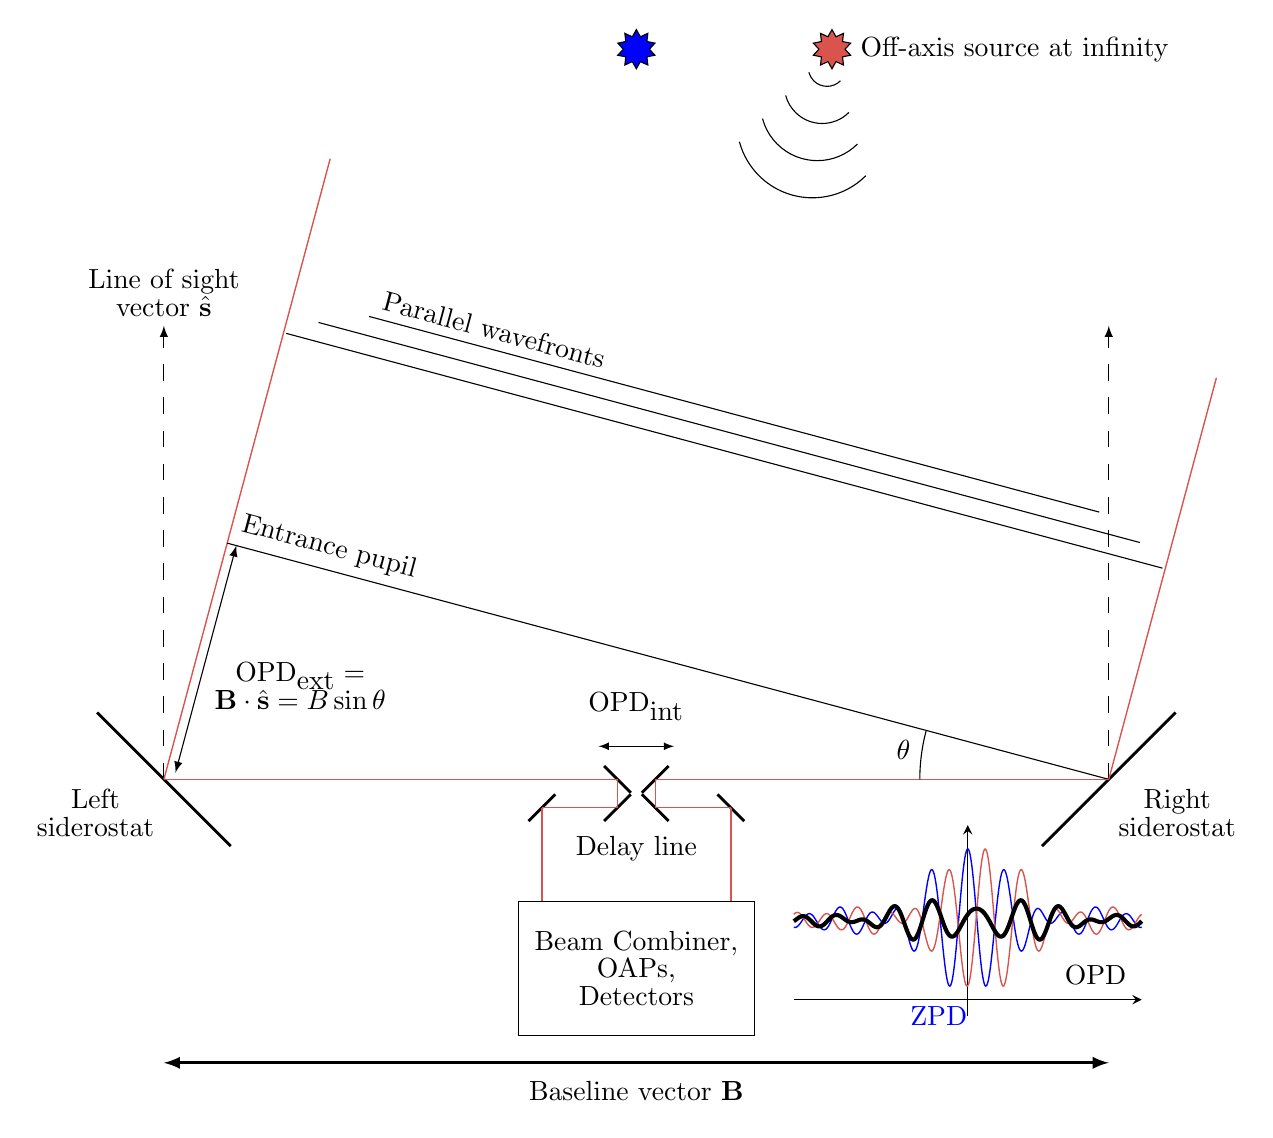
\begin{tikzpicture}[x = 1.2 cm,y=1.2 cm]
\tikzset{>=latex}
\tikzset{font={\fontsize{10pt}{10}\selectfont}}
\linespread{1}

\definecolor{palered}{RGB}{217,84,77}




\pgfmathsetmacro{\baseline}{10}
\pgfmathsetmacro{\siderostatradius}{1}
\pgfmathsetmacro{\linelength}{4}
\pgfmathsetmacro{\tiltangle}{15}
\pgfmathsetmacro{\opticslw}{1}
\pgfmathsetmacro{\raylw}{0.5}
\pgfmathsetmacro{\arcangle}{60}
\pgfmathsetmacro{\xsize}{3}

\tikzstyle{optics} = [line width = \opticslw]
\tikzstyle{rays} = [line width = \raylw,palered]


% draw siderostats
\coordinate (O) at (0,0);
\coordinate (L) at (-\baseline/2,0);
\coordinate (R) at (\baseline/2,0);
\begin{scope}[rotate = 45,shift = {(L)}]
\draw[optics] (0,-\siderostatradius) -- (0,\siderostatradius);
\end{scope}
\begin{scope}[rotate = -45,shift = {(R)}]
\draw[optics] (0,-\siderostatradius) -- (0,\siderostatradius);
\end{scope}
\node[below left,align=center]  at (L) { Left \\   siderostat};
\node[below right,align=center]  at (R) {Right \\  siderostat};

% draw delay line and other mirrors
\pgfmathsetmacro{\delaylineradius}{0.2}
\coordinate (LDLtop) at (-.2,0);
\coordinate (RDLtop) at (.2,0);
\coordinate (LDLbot) at (-.2,-.3);
\coordinate (RDLbot) at (.2,-.3);
\coordinate (LDLpickup) at (-1,-0.3);
\coordinate (RDLpickup) at (1,-0.3);
\begin{scope}[rotate = 45,shift = {(LDLtop)}]
\draw[optics] (0,-\delaylineradius) -- (0,\delaylineradius);
\end{scope}
\begin{scope}[rotate = -45,shift = {(RDLtop)}]
\draw[optics] (0,-\delaylineradius) -- (0,\delaylineradius);
\end{scope}
\begin{scope}[rotate = -45,shift = {(LDLbot)}]
\draw[optics] (0,-\delaylineradius) -- (0,\delaylineradius);
\end{scope}
\begin{scope}[rotate = 45,shift = {(RDLbot)}]
\draw[optics] (0,-\delaylineradius) -- (0,\delaylineradius);
\end{scope}
\draw[<->,line width = 0.3] (-0.4,0.35) -- (0.4,0.35)node[above=0.2cm,midway,align=center]{$\textrm{OPD}_\textrm{int}$};
\node[below] at (0,-0.5){ Delay line};
\begin{scope}[rotate = -45,shift = {(LDLpickup)}]
\draw[optics] (0,-\delaylineradius) -- (0,\delaylineradius);
\end{scope}
\begin{scope}[rotate = 45,shift = {(RDLpickup)}]
\draw[optics] (0,-\delaylineradius) -- (0,\delaylineradius);
\end{scope}

% draw vertical lines
\draw[dash pattern=on 6pt off 6pt,->] (L) -- ($(L) + (0,\linelength*1.2)$)node[above,align=center]{Line of sight \\ vector $\hat{\vectors{s}}$};
\draw[dash pattern=on 6pt off 6pt,->] (R) -- ($(R) + (0,\linelength*1.2)$);

% draw tilted vertical lines
\begin{scope}[rotate = -\tiltangle,shift = {(L)}]
\draw[rays] (0,0) -- (0,\linelength*1.7)node[pos=0.15,right=0.2cm,align=center,black]{ $\textrm{OPD}_\textrm{ext}=$ \\ $\vectors{B}\cdot\hat{\vectors{s}} = B\sin\theta$} ;
\pgfmathsetmacro{\OPD}{\baseline*sin(\tiltangle)}
\draw[<->] (0.1,0.1) -- (0.1,\OPD);
\end{scope}
\begin{scope}[rotate = -\tiltangle,shift = {(R)}]
\draw[rays] (0,0) -- (0,\linelength*1.1);
\end{scope}

% draw source
\begin{scope}[rotate = -\tiltangle]
\node[draw=black,fill=palered,star,star points=10,minimum size=0.2cm] (star) at (0,\linelength*2) {};
\node[right=0.2] at (star) {Off-axis source at infinity};
\end{scope}
\pgfmathsetmacro{\t}{\linelength*2*cos(\tiltangle)}

\node[draw=black,fill=blue,star,star points=10,minimum size=0.2cm] (starm) at (0,\t) {};


% draw wavefronts
\begin{scope}[rotate = -\tiltangle,shift={(star)}]
\draw ([shift=(-90+\arcangle:0.2)]0,-0.2) arc (-90+\arcangle:-90-\arcangle:0.2);
\draw ([shift=(-90+\arcangle:0.4)]0,-0.4) arc (-90+\arcangle:-90-\arcangle:0.4);
\draw ([shift=(-90+\arcangle:0.6)]0,-0.6) arc (-90+\arcangle:-90-\arcangle:0.6);
\draw ([shift=(-90+\arcangle:0.8)]0,-0.8) arc (-90+\arcangle:-90-\arcangle:0.8);
\draw (-\baseline/2+1,-4)node[above right,rotate = -\tiltangle]{  Parallel wavefronts} -- (\baseline/2-1,-4);
\draw (-\baseline/2+0.5,-4.2) -- (\baseline/2-0.5,-4.2);
\draw (-\baseline/2+0.2,-4.4) -- (\baseline/2-0.2,-4.4);
\end{scope}
% last wavefront
\begin{scope}[rotate = -\tiltangle,shift={(R)}]
\pgfmathsetmacro{\lengthrotatedbaseline}{\baseline*cos(\tiltangle)}
\draw (-\lengthrotatedbaseline,0)node[above right,rotate = -\tiltangle]{ Entrance pupil} -- (0,0);
\end{scope}

% draw light coming through the delay line
\draw[rays] (L) -- (LDLtop);
\draw[rays] (LDLtop) -- (LDLbot);
\draw[rays] (LDLbot) -- (LDLpickup);
\draw[rays] (LDLpickup) -- ($(LDLpickup) + (0,-1)$);
\draw[rays] (R) -- (RDLtop);
\draw[rays] (RDLtop) -- (RDLbot);
\draw[rays] (RDLbot) -- (RDLpickup);
\draw[rays] (RDLpickup) -- ($(RDLpickup) + (0,-1)$);

% draw combiner block
\node[draw,rectangle,minimum height=1.7cm,minimum width=3cm,align=center] at (0,-2) {Beam Combiner, \\ OAPs, \\ Detectors};

% draw baseline vector
\draw[<->, line width =1] (-\baseline/2,-3) -- (\baseline/2,-3)node[midway,below=0.1cm]{Baseline vector $\vectors{B}$};

% draw pointing angle
\draw ([shift=(180:2)]R) arc (180:180-\tiltangle:2) node[above left,pos=0.2]{$\theta$};

\pgfplotsset{every axis/.append style={line width=0.5pt}}
\begin{axis}[
%colormap name=hot,
%cycle list={[of colormap]},
  at = {(2cm,-3cm)},
  height=4cm,
  width=6cm,
  axis lines=middle,
%grid=major,
  clip=false,
  ymin=-0.1,
  ymax = 1.1,
  xmax = 5,
  xmin = -5,
  xlabel = {OPD},
%  ylabel = {Intensity modulation},
  xticklabels=\empty,
  yticklabels=\empty,
  legend pos=north west,
  ticks=none,
  every axis x label/.style={at={(current axis.right of origin)},anchor=north east,above left=0.1cm},
  every axis y label/.style={at={(current axis.north)},above=0.1cm},
]

\xdef\interfero{}
\foreach \m in {0.8,0.9,...,1.2} {
	\xdef\interfero{\interfero+0.5*cos(1000/\xsize*\m*x)/(1.3-0.8)*0.1}
}
\xdef\interferos{}
\foreach \m in {0.8,0.9,...,1.2} {
	\xdef\interferos{\interferos+0.5*cos(1000/\xsize*\m*(x-0.5))/(1.3-0.8)*0.1}
}
% plot sum
\addplot[black,mark=none,samples=400,line width=0.5,blue] {0.5*\interfero+0.5};
\addplot[black,mark=none,samples=400,line width=0.5,palered] {0.5*\interferos+0.5};
\addplot[black,mark=none,samples=400,line width=1.5] {0.5*\interferos+0.5*\interfero+0.5};

\end{axis}
\node[color=blue] at (3.2,-2.5){ZPD};



\end{tikzpicture}


\end{document}